\documentclass[leqno]{article}
\usepackage[utf8]{inputenc}
\usepackage[margin=2cm]{geometry}
\usepackage{fullpage,enumitem,amssymb,amsmath,xcolor,cancel,gensymb,hyperref,graphicx, multicol}
\usepackage{indentfirst, multirow, subcaption}
\setlength{\parskip}{1em}
\usepackage{float}
\usepackage{booktabs}   % professional-quality tables
\bibliographystyle{plain}
\usepackage[title]{appendix}
\usepackage[
    backend=biber,
    style=alphabetic,
    sorting=ynt
]{biblatex}
\addbibresource{refs.bib}

% Configurations for python code listing
\usepackage{listings}
\usepackage{xcolor}

\definecolor{codegreen}{rgb}{0,0.6,0}
\definecolor{codegray}{rgb}{0.5,0.5,0.5}
\definecolor{codepurple}{rgb}{0.58,0,0.82}
\definecolor{backcolour}{rgb}{0.95,0.95,0.92}
\lstdefinestyle{mystyle}{
    backgroundcolor=\color{backcolour},   
    commentstyle=\color{codegreen},
    keywordstyle=\color{magenta},
    numberstyle=\tiny\color{codegray},
    stringstyle=\color{codepurple},
    basicstyle=\ttfamily\footnotesize,
    breakatwhitespace=false,         
    breaklines=true,                 
    captionpos=b,                    
    keepspaces=true,                 
    numbers=left,                    
    numbersep=5pt,                  
    showspaces=false,                
    showstringspaces=false,
    showtabs=false,                  
    tabsize=2
}
\usepackage{xcolor}
\usepackage{listings}
\usepackage{bera}
\colorlet{punct}{red!60!black}
\definecolor{background}{HTML}{EEEEEE}
\definecolor{delim}{RGB}{20,105,176}
\colorlet{numb}{magenta!60!black}
\lstdefinelanguage{json}{
    basicstyle=\normalfont\ttfamily,
    numbers=left,
    numberstyle=\scriptsize,
    stepnumber=1,
    numbersep=8pt,
    showstringspaces=false,
    breaklines=true,
    frame=lines,
    backgroundcolor=\color{background},
    literate=
     *{0}{{{\color{numb}0}}}{1}
      {1}{{{\color{numb}1}}}{1}
      {2}{{{\color{numb}2}}}{1}
      {3}{{{\color{numb}3}}}{1}
      {4}{{{\color{numb}4}}}{1}
      {5}{{{\color{numb}5}}}{1}
      {6}{{{\color{numb}6}}}{1}
      {7}{{{\color{numb}7}}}{1}
      {8}{{{\color{numb}8}}}{1}
      {9}{{{\color{numb}9}}}{1}
      {:}{{{\color{punct}{:}}}}{1}
      {,}{{{\color{punct}{,}}}}{1}
      {\{}{{{\color{delim}{\{}}}}{1}
      {\}}{{{\color{delim}{\}}}}}{1}
      {[}{{{\color{delim}{[}}}}{1}
      {]}{{{\color{delim}{]}}}}{1},
}
\hypersetup{
    colorlinks=true,
    linkcolor=blue,
    filecolor=magenta,      
    urlcolor=cyan,
    pdftitle={Overleaf Example},
    pdfpagemode=FullScreen,
    }

\lstset{style=mystyle}
% ---------------------------------------

\title{Deep Reinforcement Learning}
\author{Nadav Shaked (312494925) and Michael Glustein (203929500)\\\texttt{\{nadav.shaked, michael.glustein\}@post.idc.ac.il}}
 
\date{July 20th, 2022}

\usepackage{mathtools}
\DeclarePairedDelimiter\floor{\lfloor}{\rfloor}

\begin{document}

\maketitle

\begin{multicols}{2}

\section{Background}
As requested in the assignment we implemented deep reinforcement models to train an agent to navigate it's car in a road environment without hitting other cars at maximum speed. The agent was trained and evaluated in three environments; a normal highway environment, a situation of a merging lane and a roundabout. We implemented in tersorflow Keras the following models; DQN, DDQN, D3QN, PPO and evaluated each one in the environments. 
The code could be found in this \href{https://colab.research.google.com/drive/1Awk9ir5vNH0lU9QfFHtts8kOa7n6V4tN?usp=sharing}{colab}.

\section{Motivation}
Reinforcement learning is an up and coming learning paradigm for decision making with uncertainty. The RL algorithm operates in an environment with limited knowledge and feedback on it's decisions. Using a reward system, the agent learns to navigate through the environment, whilst trying to maximize it's rewards, and learns the best decision. For this reason, the RL models are could be very useful for an environment like a highway. This environment has many levels of uncertainty with many unfamiliar and changing states. When trained correctly, the agent learns to navigate safely through dense roads and complicated situations. This project's purpose is to explore the learning capabilities of multiple deep reinforcement learning algorithms on the environment and evaluate them.

\section{Related Work}
\subsection{Deep Q-learning}
Interest in deep reinforcement learning grew in the 80's along with interest in neural networks, but the first breakthrough came in 2013 when DeepMind technologies published \cite{dqn} where they trained an agent using DQN to play the video game using a deep convolutional neural network. In 2015 DDQN \cite{ddqn} was developed also by DeepMind, as an off-policy algorithm, where a different policy is used for value evaluation then the policy used to select the next action. This was to correct overestimation of action values in noisy environments. D3QN \cite{d3qn} is another enhancement where the last module of the network combines the state-value and advantage outputs.

\subsection{Actor-Critic}
Many advancements and enhancements have came afterwords, for example, the Actor-Critic methods uses two neural networks, the "Actor" updates the policy distribution in the direction suggested by the Critic, and the Critic estimates the value function, either action-value or state-value.


Proximal Policy Optimization (PPO) is an alternate algorithm which optimizes “surrogate” objective function by using a stochastic gradient ascent, while using the actor-critic approach. It is called a policy gradient method, and is an enhancemant to Trust Region Policy Optimization (TRPO) also suggested by Schulman (in 2015), which limits the policy gradient step so that it doesn't move away too far from the original policy. In comparison to the traditional Q-learning algorithm, PPO is more robust and scalable. The PPO method proposes a new objective by clipping the probability ratio that forms a pessimistic estimation of the policy’s performance. Denote $r(\theta)=\frac{\pi_{\theta}(a_{t}|s_{t})}{\pi_{\theta_{old}}(a_{t}|s_{t})}$, the ratio between the value of the action under the current policy $(\theta)$ and the value of the action at state t under the previous policy ($\theta_{old}$). PPO maximizes the "surrogate" objective
\begin{equation*}
L^{CLIP}(\theta) = \hat{E}_{t}[min(r_{t}(\theta)\hat{A}_{t},clip(r_{t}(\theta), 1-\epsilon, 1+\epsilon)\hat{A}_{t})]    
\end{equation*}
where $\epsilon$ is configured as a hyper-parameter. The motivation for this objective is as follows, the left term is the TRPO maximization objective, and the right term is clipping the probability ration between $1-\epsilon$ and $1\epsilon$ which prevents $r(\theta)$ exploitation. Eventually, the algorithm calculates the pessimistic bound (lower bound) of the objective.
PPO was proposed by OpenAI and here is their algorithm taken from the research \cite{ppo}.

\begin{figure}[H]
\centering
    \centering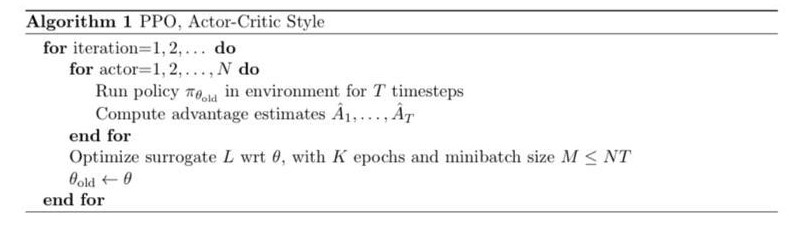
\includegraphics[width=7cm]{figs/PPO_algorithm.jpeg}
    \caption{PPO Algorithm}
  \label{ppo_algo}
\end{figure}

\section{Method}
In this project we used gym's \href{https://highway-env.readthedocs.io/en/latest/index.html}{highway} environment as our learning environment. The agents observation is 4 images of size (128, 128) to catch velocity and spatial awareness as an input. The agent chooses an action from a discrete set of actions that best fits it's policy, initialized to random. The environment also complies with a stochastic policy of 15\%. The agent is rewarded in a positive ratio to velocity with a weighted negative reward for crashing into other vehicles. Using images as input to a neural network requires initial layers of convolution and adjustments, we took inspiration from AlexNet \cite{alexnet}, using 2D convolution layers added on our model image input, in addition to the fully connected layers. This is done to scale down the number of parameters and keep the most viable information while keeping spatial information as well. The number of convolution layers and the kernel size and other parameters of each layer was subject to our consideration. When designing the model, we took into consideration key principles of convolutional networking, such as balancing depth and width of the network, elimination of representational bottlenecks and downsizing the convolutional size by layers. We normalized the image to have values between 0 and 1 to ease the training process. We used an Adam optimizer with a learning rate as a hyperparameter different for each model. We used "Mean Square Error" as our loss function as we found it to be more efficient than "Categorical Cross Entropy" and other loss functions. For all our models we created a replay memory that stored the latest transitions and sampled randomly batches of transitions that we used to train at each step.

For the DQN model, we built a neural network of three convolutional layers: the first gets an input of 4 images (128x128) in grayscale, and uses a kernel size of (8x8), stride of 4 and depth of 32. The second has a kernel of size (5x5) stride 2 and depth 64. The third has a kernel of (4x4), stride of 1 and depth of 64. All layers are linear activated. We do not use pooling layers, to not lose from the spatial information. We then flatten the image and add two fully connected linear activated layers, with a final output of the action size, that return the probability of each action. In the following figure an example of the model architecture is shown.

\begin{figure}[H]
\centering
    \centering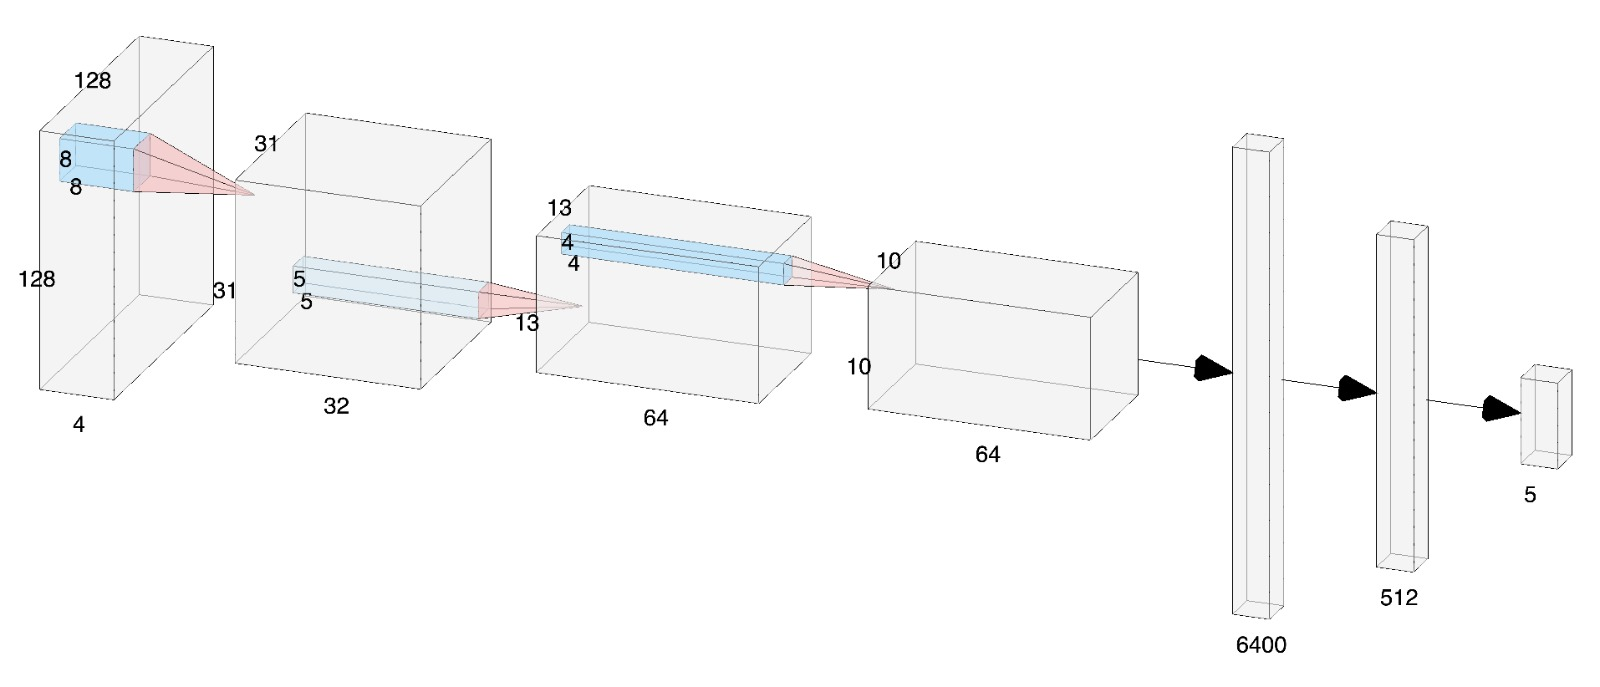
\includegraphics[width=7cm]{figs/img1.jpeg}
    \caption{Example of Model Layer Architecture - DQN}
  \label{architecture}
\end{figure}

The DDQN uses the same network, with adjustments to the training functions, while the D3QN additionally adds a final layer to the network that combines the state values and advantages to get the q-values.

For the PPO model, we implemented both an Actor and a Critic neural network. The Actor model takes as input the four images of size (128x128) in grayscale and also has three convolution layers with the same convolution parameters as DQN. The actor also takes as an input the advantage and the previous prediction to be used in it's loss function. The Critic gets just the images as input and runs the same convolution layers as well, however the critics output is just one value representing the predicted value that is used to calculate the advantage and as an input to the actors loss calculation.

An important point to mention is determining how to evaluate the model, it is not enough to just measure how many steps the agent manages to run an iteration, because also a still car could "run" forever. Measuring by rewards solely, also is not a great evaluation, because the sum of rewards is dependant on the steps the agent ran. Measuring reward/step is a better evaluation, as it helps truly evaluating the reward, however this alone is also not enough. We would like to propose a method of evaluation as follows:
\begin{equation*}
Eval = c_{1}\frac{steps}{N} + c_{2}\frac{rewards}{steps} \tag{4.1}\label{eq:4.1}
\end{equation*}
where $c_{1}$ and $c_{2}$ are coefficients we set to 0.15, 0.85 respectively, and the number of steps and rewards are the average over 100 iterations. N represents the maximum steps possible. Here we give more weight to the rewards per step but also take into consideration the number of steps the agent took, in proportion to the max amount we limited him to.

\section{Results}
\subsection{Hyper-parameters}
Before we began we decided to examine the influence of the hyper-parameters to chose parameters that will maximize performance. We compared two learning rates: 1e-4 and 5e-5, the higher the value, the more likely the algorithm is to reach a local optimum area, the lower value should take longer training but eventually give better results. We also examined two initial exploration probabilities 0.2 and 0.35, the higher the probability, the policy algorithm should ignore the models action prediction and select in random, which increases the exploration of uncommon states and could be more efficient in our game, it should slow down convergence. We tested the combination of the different parameters and plotted the results.

\begin{figure}[H]
  \begin{tabular}{ll}
    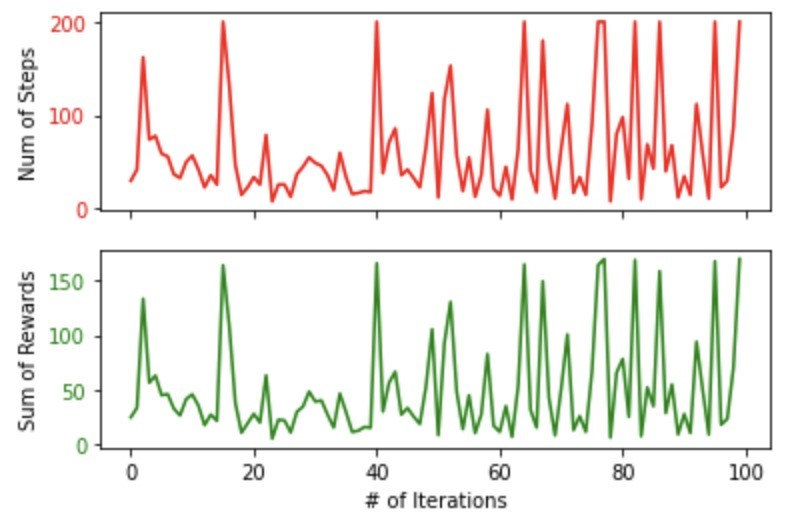
\includegraphics[scale=0.18]{figs/hyp_lr4_exp2.jpeg}&
    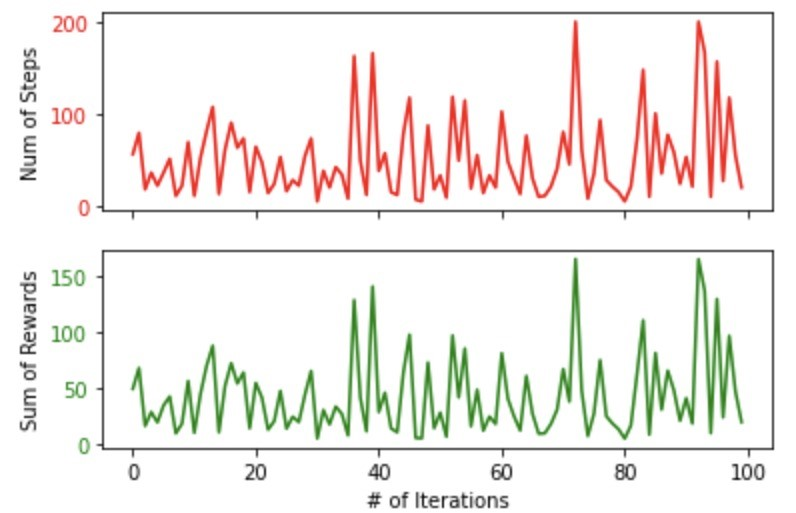
\includegraphics[scale=0.18]{figs/hyp_lr4_exp3.jpeg}\\
    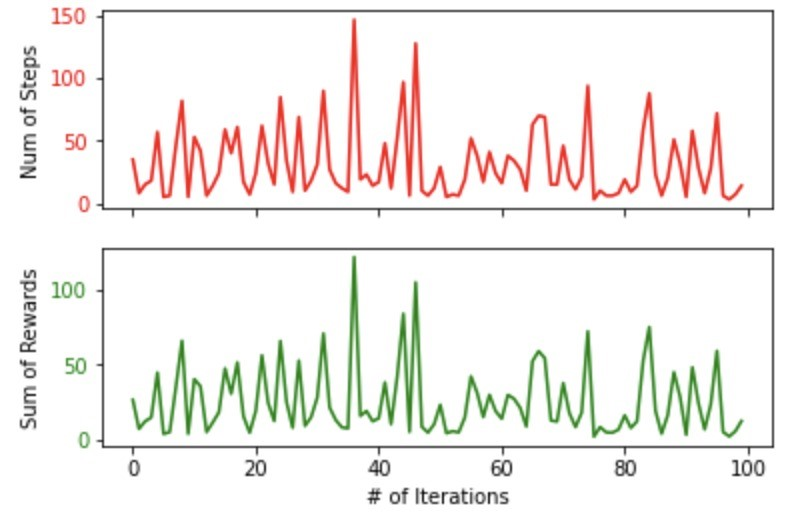
\includegraphics[scale=0.18]{figs/hyp_lr5_exp2.jpeg}&
    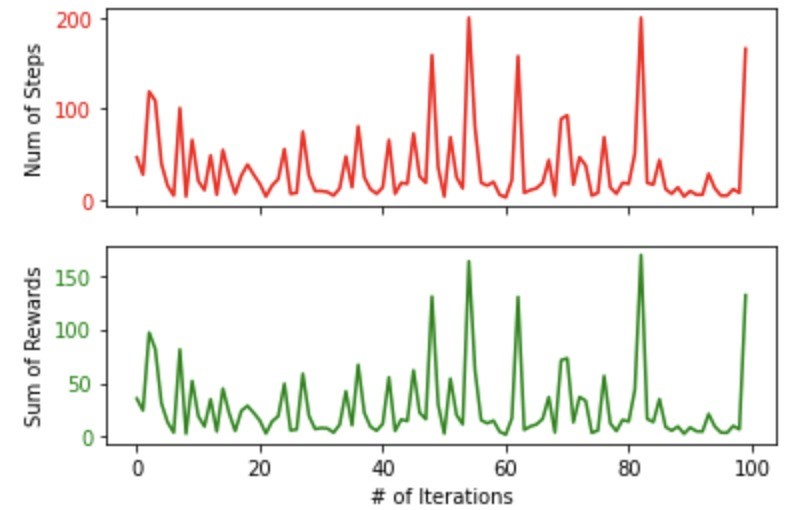
\includegraphics[scale=0.18]{figs/hyp_lr5_exp3.jpeg}\\
  \end{tabular}
  \caption{Top-left: lr=1e-4, expl=0.2. Top-right:lr=1e-4, expl=0.35. Bottom-left:lr=5e-5, expl=0.2. Bottom-right:lr=5e-5, expl=0.35}
  \label{hyperparams}
\end{figure}

\begin{tabular}{ |p{3.5cm}|p{2.5cm}|}
 \hline
 Params & Reward / Step\\
 \hline
 \hline
 LR 1e-4, Expl 0.2 & 0.78\\
 LR 1e-4, Expl 0.35 & 0.71\\
 LR 1e-5, Expl 0.2 & 0.72\\
 LR 1e-5, Expl 0.35 & 0.71\\
 \hline
\end{tabular}
\captionof{table}{Hyper-parameter evaluation}

We expected the best results to be with the lower learning rate and higher exploration, but we received the opposite. Our assumption for this result is the relative low number of epochs in the training session, the smaller learning rate reaches a local optimum faster and therefore performs better overall. Regarding exploration, the environments stochastic policy of 15\% adds it's own "exploration" and thus too much exploration could manipulate the results, not allowing the model to build a proper policy. For this reason, we decided to train our models with learning rate of 1e-4 and initial exploration of 20\%. We added an exploration decay, to allow the model to "listen" more to it's policy as it is more trained and mature.

\subsection{Ex1 - Highway environment}
In the first exercise, we trained all of our models on the highway environment with the first configuration, with the following hyper-parameters:
\begin{lstlisting}
learning rate: 1e-4,
initial exploration: 20%,
exploration decay: 0.99 (every 20 epochs),
mini batch size: 64
\end{lstlisting}
In deep RL, as opposed to other learning models we do not have a "ground truth". In each model we calculate the loss a little differently, but mostly it is the difference between the expected reward and the actual reward. We update our policy by minimizing the loss and ultimately maximizing the rewards. During the training we saved the loss history of the model, and the reward history. The loss history doesn't reveal much information to us but it is used by the model to "correct" the policy, however we expect the rewards to grow with the training. It should be noted, that we trained the model in multiple runs, and the "replay memory" was not saved between runs, this adds some zeros to the loss graph.
\begin{figure}[H]
\centering
  \begin{subfigure}{8cm}
    \centering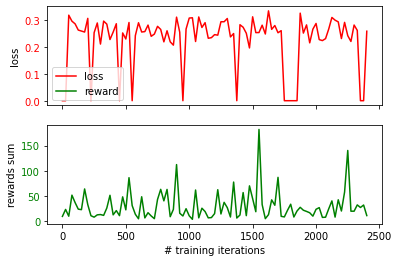
\includegraphics[width=7cm]{figs/ddqn_ex1_loss.png}
    \caption{Loss history and sum of rewards per iteration of the DDQN model during training}
  \end{subfigure}
% \end{figure}%
% \begin{figure}[H]\ContinuedFloat
  \begin{subfigure}{8cm}
    \centering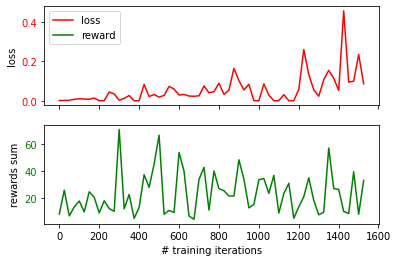
\includegraphics[width=7cm]{figs/d3qn_ex1_loss.png}
    \caption{Loss history and sum of rewards per iteration of the D3QN model during training}
  \end{subfigure}
  \caption{Exercise 1 - Training}
\end{figure}
 After the training we ran 100 iterations of a full game, with a limit of 200 steps a round. Here is a plot of the sum of rewards per iteration and of the number of steps an iteration.

\begin{figure}[H]
\centering
  \begin{subfigure}{8cm}
    \centering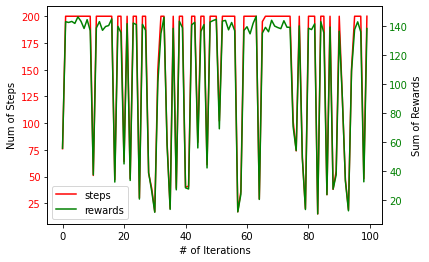
\includegraphics[width=7cm]{figs/ddqn_ex1_100_iters.png}
    \caption{DDQN Rewards and Steps per 100 iterations}
  \end{subfigure}
\end{figure}%
\begin{figure}[H]\ContinuedFloat
  \begin{subfigure}{8cm}
    \centering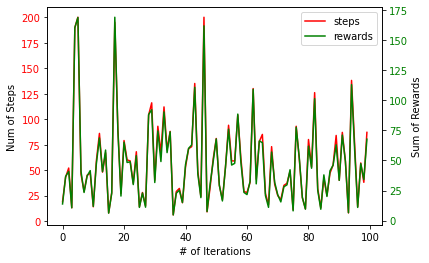
\includegraphics[width=7cm]{figs/d3qn_ex1_100_iters.png}
    \caption{D3QN Rewards and Steps per 100 iterations}
  \end{subfigure}
% \end{figure}%
% \begin{figure}[H]\ContinuedFloat
  \begin{subfigure}{8cm}
    \centering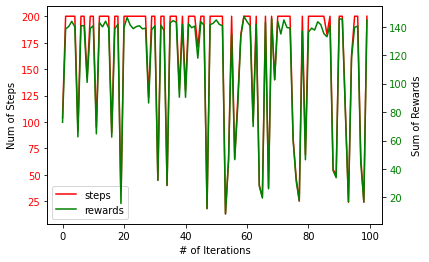
\includegraphics[width=7cm]{figs/ppo_ex1_100_iters.png}
    \caption{PPO Rewards and Steps per 100 iterations}
  \end{subfigure}
  \caption{Exercise 1 - Evaluation}
%   \label{ex1}
\end{figure}


In summary, the average rewards and steps are shown in the table below. We also calculated the average reward per step. Note: we limited the run to 200 steps.

\begin{tabular}{ |p{1cm}||p{1.5cm}|p{1.5cm}|p{1.2cm}|p{1cm}|  }
 \hline
 Model&Average Steps& Average Rewards& Reward / Step&Eval\\
 \hline
 DDQN & 151.13 & 106.05 & 0.7 & 0.7\\
 D3QN & 58.26 & 47.78 & 0.82 & 0.72\\
 PPO & 159.01 &112.04 &  0.7 & 0.71\\
 \hline
\end{tabular}
\captionof{table}{Exercise 1 - Summary}

\subsection{Ex2 - Aggressive Environment}

We continued training the models on the highway environment with configuration 2, which is a more aggressive environment, with more lanes and more cars and more density. We used the same hyper-parameters as exercise 1. After training, we again ran each model for 100 iterations and plotted the steps and rewards per iteration to evaluate the models.

\begin{figure}[H]
\centering
  \begin{subfigure}{8cm}
    \centering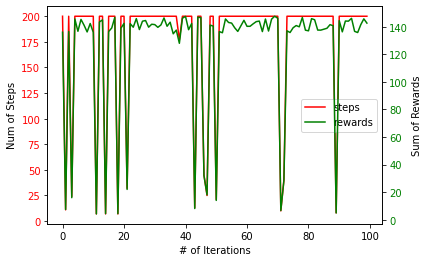
\includegraphics[width=7cm]{figs/ddqn_ex2_100_iters.png}
    \caption{DDQN Rewards and Steps per 100 iterations}
  \end{subfigure}
%  \end{figure}%
% \begin{figure}[H]\ContinuedFloat
  \begin{subfigure}{8cm}
    \centering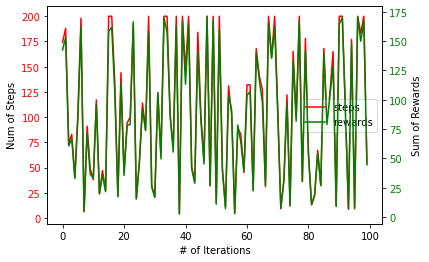
\includegraphics[width=7cm]{figs/d3qn_ex2_100_iters.png}
    \caption{D3QN Rewards and Steps per 100 iterations}
  \end{subfigure}
%  \end{figure}%
% \begin{figure}[H]\ContinuedFloat
  \begin{subfigure}{8cm}
    \centering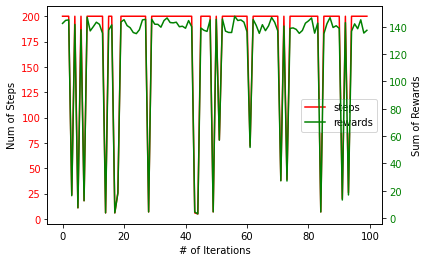
\includegraphics[width=7cm]{figs/ppo_ex2_100_iters.png}
    \caption{PPO Rewards and Steps per 100 iterations}
  \end{subfigure}
  \caption{Exercise 2 - Evaluation}
%   \label{ex2}
\end{figure}

Here are the average results and evaluation of the models.\\

\begin{tabular}{ |p{1cm}||p{1.5cm}|p{1.5cm}|p{1.2cm}|p{0.8cm}|  }
 \hline
 Model&Average Steps& Average Rewards& Reward / Step&Eval\\
 \hline
 DDQN & 176.27 & 124.48 & 0.7 & 0.73\\
 D3QN & 104.13 & 85.08 & 0.81 & 0.77\\
 PPO & 169.96 & 119.76 &  0.7 & 0.72\\
 \hline
\end{tabular}
\captionof{table}{Exercise 2 - Summary}


\subsection{Ex3 - Super Agent}

In this section, we trained our models on multiple environments, highway, merge and roundabout, while switching between them. We switched every 500 - 1000 epochs (and not in a random manner), so that the replay memory could have enough time to get "filled" with relevant data (transitions) to the trained environment and learn to make relevant decisions. We "emptied" the replay memory before changing environments, so that it won't have a negative affect on the training, where the agent learns wrong policies. We limited the highway environment to 200 steps a game, and the merge and roundabout environment to 50, we found that the environment "ends" after that and we don't gain much information.

\begin{figure}[H]
\centering
%   \begin{subfigure}{8cm}
%     \centering
\includegraphics[width=7cm]{figs/placeholder.png}
%     \caption{Loss history and sum of rewards per iteration of the D3QN model during training}
%   \end{subfigure}
% \end{figure}%
% \begin{figure}[H]\ContinuedFloat
%   \begin{subfigure}{8cm}
    \centering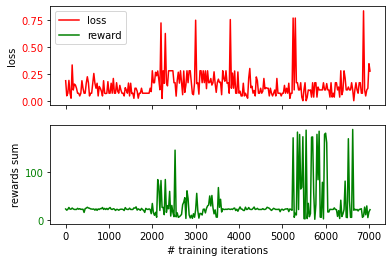
\includegraphics[width=7cm]{figs/ppo_ex3_loss.png}
    \caption{Loss history and sum of rewards per iteration of the PPO model during training}
%   \end{subfigure}
%   \caption{Exercise 3 - Training}
\end{figure}

In the training graphs, we could see the difference between environments very clearly. Since the merge and roundabout envs were limited to 50 steps, their rewards is also limited. For example, in PPO, the area in the graph between 2k-3k and 5k-7k belong to the highway environment (which is limited at 200 steps). We could see a very large increase in the rewards between both training sessions.

\subsubsection{Highway}

\begin{figure}[H]
  \begin{tabular}{ll}
    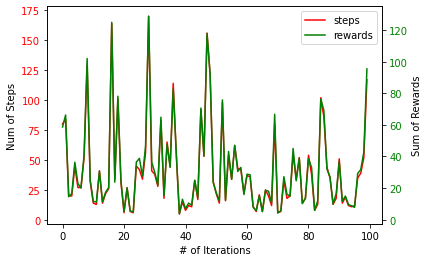
\includegraphics[scale=0.25]{figs/d3qn_ex3_highway.png}&
    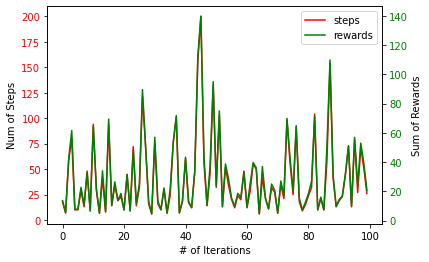
\includegraphics[scale=0.25]{figs/ppo_ex3_highway.png}\\
  \end{tabular}
  \caption{Rewards and Steps per 100 iterations on highway env. Left: D3QN. Right: PPO}
  \label{hyperparams}
\end{figure}


Here are the average results and evaluation of the models.\\

\begin{tabular}{ |p{1cm}||p{1.5cm}|p{1.5cm}|p{1.2cm}|p{0.8cm}|  }
 \hline
 Model&Average Steps& Average Rewards& Reward / Step&Eval\\
 \hline
 D3QN & 41.02 & 31.99 & 0.78 & 0.66\\
 PPO & 40.6 & 30.12 & 0.74 & 0.63\\
 \hline
\end{tabular}
\captionof{table}{Exercise 3 - Highway Summary}

\subsubsection{Merge}

\begin{figure}[H]
  \begin{tabular}{ll}
    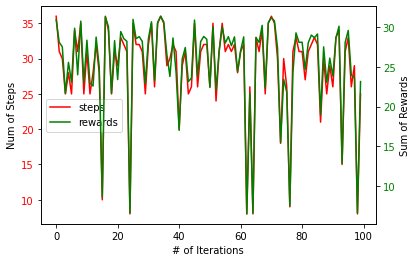
\includegraphics[scale=0.25]{figs/d3qn_ex3_merge.png}&
    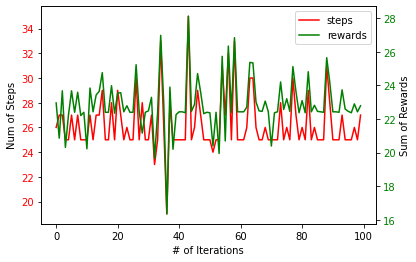
\includegraphics[scale=0.25]{figs/ppo_ex3_merge.png}\\
  \end{tabular}
  \caption{Rewards and Steps per 100 iterations on merge env. Left: D3QN. Right: PPO}
  \label{hyperparams}
\end{figure}

Here are the average results and evaluation of the models.\\

\begin{tabular}{ |p{1cm}||p{1.5cm}|p{1.5cm}|p{1.2cm}|p{0.8cm}|  }
 \hline
 Model&Average Steps& Average Rewards& Reward / Step&Eval\\
 \hline
 D3QN & 28.74 & 25.33 & 0.88 & 0.86\\
 PPO & 26.26 & 22.85 &  0.87 & 0.85\\
 \hline
\end{tabular}
\captionof{table}{Exercise 3 - Merge Summary}

\subsubsection{Roundabout}

\begin{figure}[H]
  \begin{tabular}{ll}
    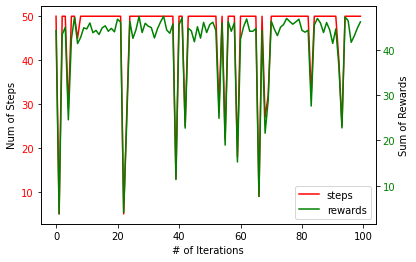
\includegraphics[scale=0.25]{figs/d3qn_ex3_roundabout.png}&
    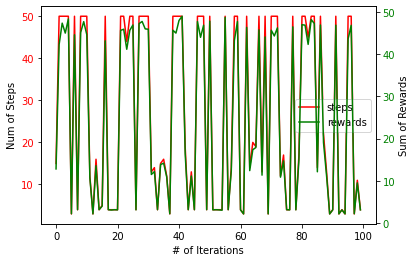
\includegraphics[scale=0.25]{figs/ppo_ex3_roundabout.png}\\
  \end{tabular}
  \caption{Rewards and Steps per 100 iterations on \textbf{roundabout} env. Left: D3QN. Right: PPO}
  \label{hyperparams}
\end{figure}

Here are the average results and evaluation of the models.\\

\begin{tabular}{ |p{1cm}||p{1.5cm}|p{1.5cm}|p{1.2cm}|p{0.8cm}|  }
 \hline
 Model&Average Steps& Average Rewards& Reward / Step&Eval\\
 \hline
 D3QN & 45.84 & 41.08 & 0.89 & 0.89\\
 PPO & 26.94 & 24.55 & 0.91 & 0.85\\
 \hline
\end{tabular}
\captionof{table}{Exercise 3 - Roundabout Summary}


\subsubsection{Summary}

In summary let's show the evaluation according to our eval method \ref{eq:4.1} for each environment.\\

\begin{tabular}{ |p{1cm}||p{1.5cm}|p{1.2cm}|p{1.8cm}| }
 \hline
 Model&Highway& Merge& Roundabout\\
 \hline
 D3QN & 0.66 & 0.86 & 0.89 \\
 PPO & 0.63 & 0.85 & 0.85 \\
 \hline
\end{tabular}
\captionof{table}{Exercise 3 - Evaluation Summary}


\section{Conclusions}
Our first conclusion is that in order to get good results, the model must train a lot. We trained each model for over 24 hours and a few thousand epochs to get good results. Many times we have reached a "local minimum" where the model just learned to slow down or speed up. We overcame this with raising exploration and continuing to train the model for longer. It is difficult to evaluate a model with the regular loss functions or with f1 scores, since we don't have "ground truth". We discovered that to properly evaluate the model, we must take into consideration also the number of steps the agent manages to take an iteration and also the average reward. In exercise 1, in both DDQN and PPO, the agent managed averaged over 75\% of possible steps an iteration, in a stochastic environment. The D3QN agent averaged less steps (only 25\%), however it's rewards per step was much higher. In the videos seen in the colab notebook it is easy to see the DQN and PPO models slowing and reaching areas with no other drivers, while the D3QN agent maneuvers between other players. Using our evaluation method, that puts more emphasis on reward, D3QN seemed to be the better performer, with a score of 0.72.  

Our models behaved in the more aggressive environment of exercise 2 similar to the first highway environment. Both the DDQN and PPO models were more likely to finish the iteration without crashing, but drove much slower and had a lower average reward. The D3QN maneuvered nicely between cars, but crashed more often, in total, the D3QN performed best with an evaluation score of 0.77.

In the third exercise, we realized that learning on a new environment, deteriorates from the performance of other environments. Also, the model seems to always perform best on the "most recently" trained environment. To overcome this, after the bulk training of all environments, we added a few hundred iterations to each environment again. We found the multi-agent training to be much more difficult than a sole environment. The better our model got in one environment, the worse it got in another. We think that the model has to train longer on each environment separately and then together to receive better results. Our super-agent performed well at the merge and roundabout environment in both models we trained it on. D3QN performed slightly better than PPO. However, we saw a deterioration in the highway environment, where our agents performed much worse than in exercise 1 and 2.

A few improvements we wish to propose, that we think could further enhance performance. We think some modifications to the reward system may help the model overcome local maximums of "slowing down", changing the proportion to the reward per speed or adding a reward when the car overcomes another car could help.


\printbibliography

\end{multicols}

\end{document}
